\documentclass[11pt]{article}
\usepackage[utf8]{inputenc}

\usepackage[left=2.5cm,top=2.5cm,right=2.5cm,bottom=2.5cm]{geometry}
\usepackage{times} % font type
\usepackage{url} % for clickable web addresses in PDF document
\usepackage{graphicx} % for figures
\usepackage{float} % to force figure or table here [H]
\usepackage{multirow} % For tables with different rows and columns

\title{Precision medicine and quantitative imaging in glioblastoma \\ - a multiscale approach}
\author{OERCompBiomed Summer School, 10-14 August 2020\\
{\footnotesize \url{https://github.com/oercompbiomed/Seili-2020}}}


\date{Template based on the report from Group\#1 at the previous 2019 Seili Summer School\\
(for which PROSTATE CANCER was the topic)}
\begin{document}

\maketitle

\begin{scriptsize}
\begin{verbatim}
Group members:
NN, KI (n.n@stud.ki.se)
NN, SDU (nn@student.sdu.dk)
NN, SDU (nn@student.sdu.dk)
NN, UEF (nn@student.uef.fi)
\end{verbatim}
\end{scriptsize}
\vspace{8mm}
\section{Research plan} % 3-5 pages incl. figures and bibliography

\vspace{3mm}

\subsection{A brief background to the field}
Prostate cancer (PCa) is the most common form of cancer for men. Usually it grows slowly and rarely causes any symptoms on its early stage. However, in latest stages PCa can lead to urinary difficulties, blood in urine and pain in the pelvis, back and during urinating (Smith et al. 2017, Pentyala et al., 2016). Reason for lack of symptoms can be e.g. that malignancies start to grow in the peripheral portion of the prostate away from the prostatic urethra. PSA is commonly used marker in PCa screening. PSA ratio increases during cancer development due to increased epithelial cell proliferation as PSA is secreted by the epithelial cells of the prostate gland (Pentyala et al., 2016). 

Test that are now used might lead to false positive and negative diagnosis. Because of this, multiparametris MRI (mpMRI) potential as a diagnostic tool. mpMRI gives the best anatomic imaging of the prostate gland. mpMRI has two anotomic sequences, T1 and T2 weighted. T1 weighting is useful for detecting hemorrhage of the biopsy. T2 in turn provides the highest soft tissue resolution for tumor vizualization (zonal anatomy, capsule, neurovascular bundles, anterior fibrous stroma, and seminal vesicles). Decision to undergo active surveillance or treatments is based on multiple factors, like serum PSA, Gleason score and PSA density. However, mpMRI can be used when aggressiveness and risk stratification is made. (Turkbey and Choyke, 2012) Also, prostate specific membrane antigen (PSMA) can be used as a marker during prostate cancer diagnosis. PSMA is one of the most specific cell surface markers for prostate cancer diagnosis and targeted treatment. It plays important roles in many physiological processes like signal transduction, receptor function, nutrient uptake and cell migration. PSMA expression increases while androgen receptor is down regulated. This increased expression can be associated with tumor grade, pathologic state, high Gleason score and PSA recurrence. Development of PSMA-targeted protein, like ProCA32, MRI contrast agents are expected to have applications in the molecular imaging in early stages of prostate cancer and further with drug treatment effects by noninvasive evaluation of the PSMA level using MRI. (Pu et al., 2016)


\subsection{Objectives and expected impact}
\vspace{5mm}
One of the main challenges in the application of the DL to medical image analysis is the scarcity of available data for training. To address this issue the researchers started to use the combination of the CNN based DL networks and supervised feature-based decision tree to differentiate benign and malignant cancers. Liu et al. achieved AUC of 0.95 for the differentiation of the benign and malignant cancer. It was also indicated that the DL unsupervised learning outperformed the supervised learning with AUCs of 0.84 and 0.80, respectively. The data from 274 mpMRI images has been augmented, producing 207,144 image patches for the training data purposes. (Liu,2017)

To overcome the issue of the data scarcity, researchers started to test the hybrid approach, which include both supervised and unsupervised learning. Karimi et al. suggested combination of the handcrafted features with learned features for classification of prostate cancer using mpMRI. In this study the significant features were produced using CNN, handcrafted features were based on statistical data and texture. 51 features were identified and the combination of the three types of parameters allowed to differentiate benign and malignant cancer tissues with AUC of 0.87. The separate subset testing showed lower performance power of 0.70, 0.68 and 0.75 for the statistical, handcrafted and learned features respectively. (Karimi, 2017)
 

 \vspace{8mm}
 \begin{table}[H]
\begin{center}
\begin{tabular}{ |p{3cm}|p{5cm}|p{5cm}|   } 
\hline
{\bf Research} & {\bf Liu, 2017}  & {\bf Karimi, 2017}  \\ 
\hline
Number of cases&169&203 \\ 
\hline
Results&CNN based DL (0.84) vs feature-based method (0.80)&CNN-based DL handcrafted feature- based decision trees (0.87)  \\ 
 & & \\
 & & 0.75 - CNN-derived features \\
 & & 0.68 - handcrafted texture\\
 & & 0.70 - statistical features\\
 \hline
\end{tabular}
\caption{Represent the data from the research of the Competitors and inspirers Research}
\end{center}
\end{table}
 
 
 
 
 
 
 
 
 
 
 
 In this study the hybrid approach will be used to recognize the phenotypic characteristics and outperform   the clinician abilities in characterization of the prostate-cancer.
Objective/Impact: The main objective of this study is to perform prediction on the aggressiveness of the prostate-cancer and to distinguish between benign and highly aggressive malignant prostate cancer. Expectations for this algorithms are that it can be used in clinics as a part of PCa diagnostics and make it easier to decide which patient needs treatments immediately and who needs only regular follow-up or no treatment at all. 
From the economical aspect it is expected that it will reduce the expenses for the treatment as well as increasing the survival rate of the patients. Better image resolution and  can often lead to early cancer identification and further overdiagnosis in prostate cancer. Moreover, this approach will allow to identify cancer non-invasively, compared to the currently available diagnostics method in hospitals. 


\vspace{3mm}
\newpage
\subsection{Material and methods}


This study is the combination of supervised and unsupervised learning. To identify significant parameters on the MRI pictures, the deep learning autoEncoder approach will be applied using the TensorFlow library and KERAS interface. Then, the obtained highly significant features will be applied further in a supervised learning algorithm. The significant features as well as PSA, age, the state of survival after diagnosis, PSMA and Gleason score data will be input into the Random Forest algorithm to make our own model. We expect the detection of reasonable features, which will allow us to distinguish between benign, malignant and aggressive cancer types. Both control and case group will consist of males over the age of 50. 
\vspace{5mm}


\vspace{7mm}
\textbf{Unsupervised learning}
\newline
AutoEncoder neural network is an unsupervised deep learning algorithm that is composed of two parts, an encoder that compresses input data with retaining the data’s unique traits through convolutional layers and a decoder that enables to reconstruct the encoded image features close to (back to) original. In this study, the encoder part will be solely employed to extract significant features (= the encoded image features.) from the three-dimensional images.
The three-dimensional mpMRI will be used as input data for the AutoEncoder. The images including lesion are converted to image patch stacks (25 width x 25 height x 10 layers x 1 grey scale) through the convolutional layers which will be used for an input layer. Compressed data will be produced through the encoder. Then, the significant feature from each image will be obtained from the compressed data. (Hanh et al. 2018) 
AutoEncoder will be executed by a Keras which is neural network Application program interface (API) written in python.
\vspace{7mm}
\begin{figure}[H]
\centering
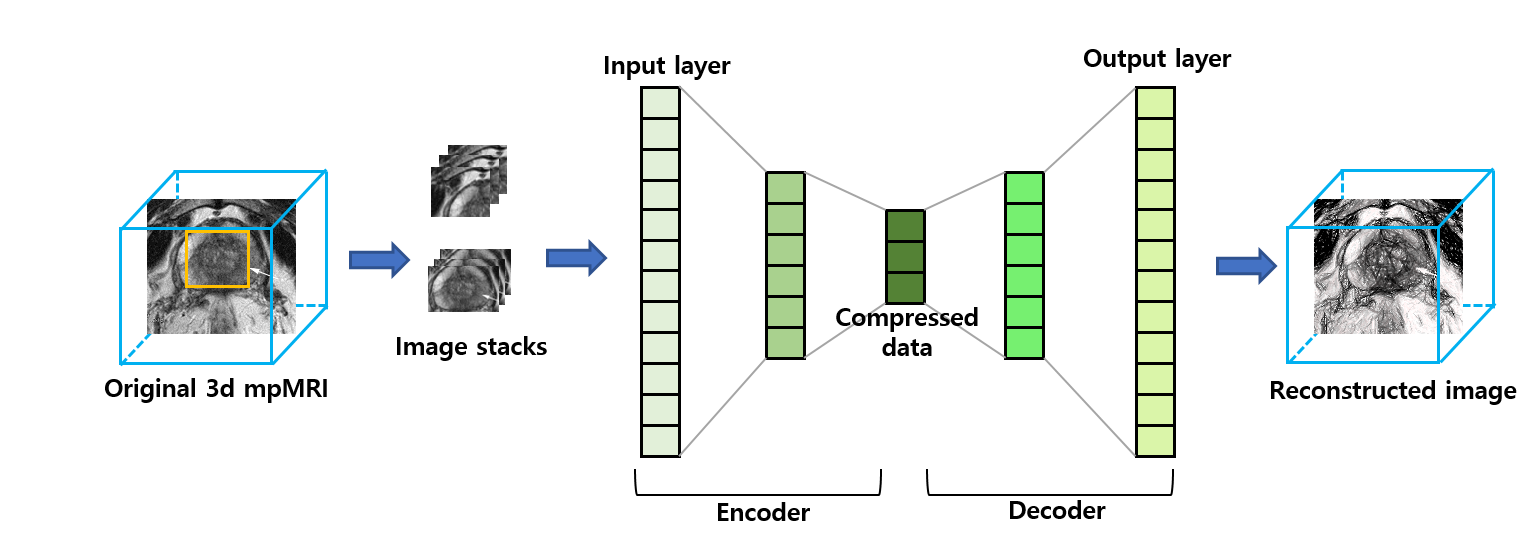
\includegraphics[width=0.98\linewidth]{Fig1_The_process_of_autoEncoder.png} 
\vspace{-3mm}
\caption{\footnotesize The process of autoEncoder
}
\label{fig:fig3}
\end{figure}

\newpage
\vspace{7mm}
\textbf{Supervised learning}
\newline
Random forest is one of the supervised learning algorithms that is made up of multiple decision trees. Each tree consists of collective nodes, where each node is divided into two nodes. In this study, we will apply the random forest algorithm to generate our prediction model. In machine learning, data often requires pre-processing steps such as normalization when parameters have various ranges or scales. But the random forest is not sensitive about the normalization of the data. So, the parameter will be used directly without any pre-processing.(Dinç et al. 2014)
Scikit-learn in python is employed for the random forest. First, training and test data are selected 80 and 20 respectively. The data set will be randomly distributed to avoid selective bias. The training data set is bootstrapped and then decision trees are created by drawing from the bootstrapped dataset. Hyper parameter tuning can be used to reduce variance. We can identify valuable attributes by computing the relative importance of each attribute from the result of random forest. The random forest will possess 4 outcomes, benign, healthy, malignant, and aggressive
\hfill \break
\vspace{5mm}

\subsection{Evaluation}
After supervised learning, the evaluation of the output can be achieved by the construction of the confusion matrix (CM), which will compare the actual “ground truth” data with the predicted data. It is also possible to test the approach on clinical patients, by comparing with the actual data. From the confusion matrix, recall,  precision, specificity and accuracy can be obtained. Recall and precision are generally used for assessment of performance of the prediction model. Both will be obtained between 0 to 1. The higher value the better. Recall is also called sensitivity, it is the  probability that data is correctly classified from total relevant results. Precision is the probability that a prediction of the state of the prostate cancer is correct. Both values have trade offs. So, for our model, we should try to have some balance between them.

\vspace{3mm}
\begin{footnotesize}

\begin{thebibliography}
{1} 
\bibitem{Chaddad2018}  Chaddad A, Niazi T, Probst S, Bladou F, Anidjar M and Bahoric B. Predicting Gleason Score of Prostate Cancer Patients Using Radiomic Analysis.
Front Oncol 2018;8:630. 
{2}
\bibitem{Smith2017} Smith Z, Eggener S and Murphy A. African-American Prostate Cancer Disparities
Curr Urol Rep 2017;18:10
{3}
\bibitem{Pentyala2016} Pentyala S, Whyard T, Pentyala S, Muller J, Pfail J, Parmar S, Helguero C.G and Khan S. Prostate cancer markers: An update
Biomed Rep 2016;4:268
{4}
\bibitem{Odongo2018} Odongo Steven Eyobu and Dong Seog Han, Feature Representation and Data Augmentation for Human Activity Classification Based on Wearable IMU Sensor Data Using a Deep LSTM Neural Network Sensors, 18:9, 2892
{5}
\bibitem{Hanh2018} Hanh Vu, Hyun-Chul Kim, and Jong-Hwan Lee, 3D convolutional neural network for feature extraction and classification of fMRI volumes, 2018 International Workshop on Pattern Recognition in Neuroimaging, Singapore, pp1-4 
{6}
\bibitem{Dinc2014} Dinc, İmren et al. Evaluation of Normalization and PCA on the Performance of Classifiers for Protein Crystallization Images. Proceedings of IEEE Southeastcon. IEEE Southeastcon vol2014
{7}
\bibitem{Turkbey and Choyke2012} Turkbey Baris and Choyke L. Peter (2012) Multiparametric MRI and prostate cancer diagnosis and risk stratification. Curr Opin Urol. 2012;22:310-315
{8}
\bibitem{Pu2016} Pu F., Salarian M., Xue S., Qiao J., Feng J., Tan S., Patel A., Li X., Mamouni K., Hekmatyar K., Zou J., Wu D., and Yang J. J. (2016) Prostate-specific membrane antigen targeted protein constrast agents for molecular imaging of prostate cancer by MRI. Nanoscale;8:12668-12682
{9}
\bibitem{Liu2017}Liu, S., Zheng, H., Feng, Y. and Li, W. (2017) Prostate cancer diagnosis using deep learning with 3D multiparametric MRI. Proc. SPIE Int . Soc. Opt. Eng. 10134, 1013428 .
{10}
\bibitem{Sandhu2012}Sandhu, Gurdarshan S, and Gerald L Andriole. “Overdiagnosis of prostate cancer.” Journal of the National Cancer Institute. Monographs vol. 2012,45 (2012): 146-51. doi:10.1093/jncimonographs/lgs031
\end{thebibliography}
\end{footnotesize}

% See also: https://www.overleaf.com/learn/latex/Bibliography_management_in_LaTeX
% considering BibTeX / Jabref / Mendeley / Zotero / EndNote
% using BibTeX you can also edit the bib file directly via the files menu

\newpage


\section{Data management plan and ethical considerations} % 1 1/2-2 1/2 pages incl. graphics / links


\subsection{Description of generated data and code}




 Data for 2000 people will be acquired from biobanks in Northern Europe (Sweden, Norway, Denmark, Finland, Iceland, the Baltic countries and the UK) and divide into two groups , a control group (1000 healthy people) and a case group (1000 patients with prostate cancer). The subgroup of the patients will be from the patients suffering from the castrate resistant prostate cancer. The 2000 images will turn into the significant features through unsupervised learning. This feature will be employed with other parameters for supervised learning to make our own model.
 
There are some possible problems caused by using different types of data and methods. It can prevent the significant changes in the performance of the approach. In unsupervised learning, we will use the images taken from different biobanks and the acquisition of the images could be different for the of mpMRI images. Even though our sample size is 2000, data augmentation in deep learning would allow us to increase the number of images by generating deformations of training data set while keeping the symbolism of data. Because of this obtained heterogeneous sample issues can be solved. (Odongo  2018) In supervised learning, all data will be split into training and test group at 80 and 20 respectively considering selection bias. For example, we have data from many different ages. Only people in their fifties may be assigned to a test group. Because of this, when we evaluate our model, the prediction will be off, to make it more accurate the model will be distributed uniformly as possible. 
% Table for parameter 
\begin{table}[H]
\begin{center}
\begin{tabular}{ |p{4cm}|p{9cm}|   } 
\hline
{\bf Parameters} & {\bf Levels}  \\ 
\hline
PSA (ng/mL) & $ 0 < PSA < 2.5, 2.5 \leq PSA < 4, 4 \leq PSA < 10, 10 \leq $ \\ 
\hline
Gleason Score & 6 to10  \\ 
\hline
 PSMA \scriptsize (prostate specific membrane antigen) & 0(absent), 1(weak), 2(moderate), and 3(strong) PSMA staining intensity \\
\hline
Age & 50 - 59, 60 - 69, $70 \leq $  \\ 
\hline
State of survival & Alive or death after five years  \\ 
\hline
\end{tabular}
\caption{The list of parameters}
\end{center}
\end{table}
\begin{figure}[H]
\centering
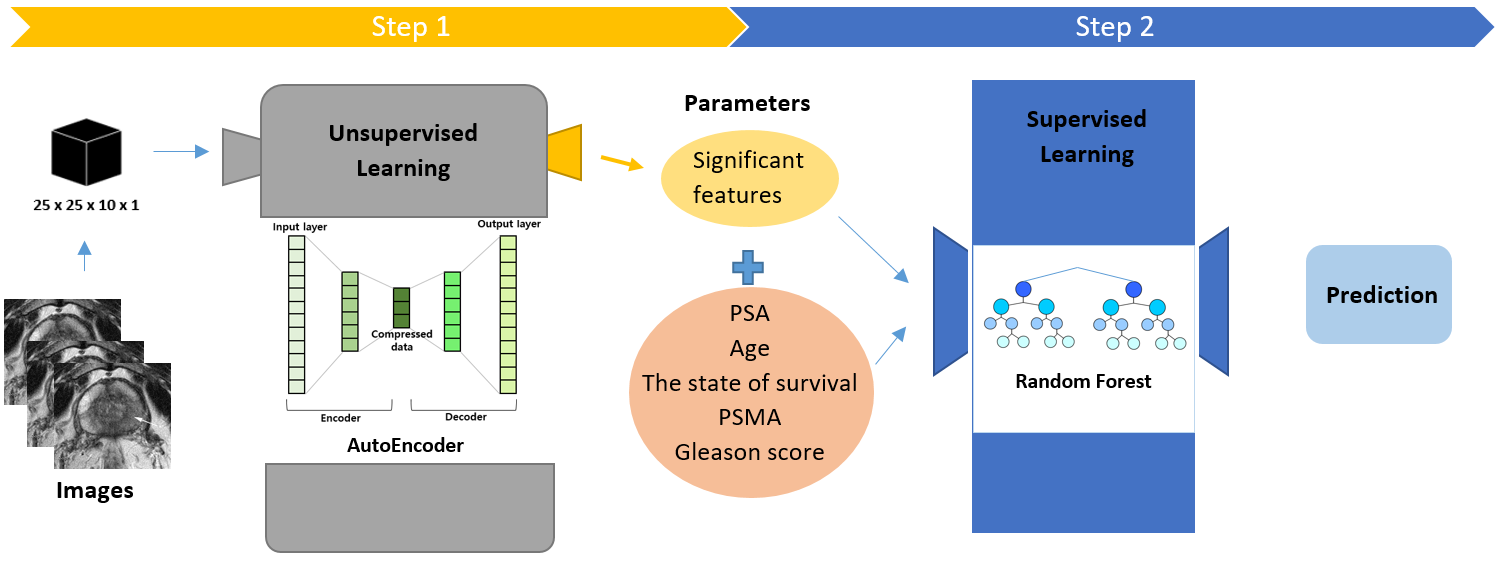
\includegraphics[width=0.98\linewidth]{Fig2_Overview_of_the_process.png} 
\vspace{-3mm}
\caption{\footnotesize The overview of the process
}
\label{fig:Fig2}
\end{figure}

\subsection{Sharing of data and code}
The code will be accessible at Bitbucket for researchers to use for further research. The data retained from this study can be obtained from the IEEE dataport, and relevant data will also be returned to the Biobank as a part of the agreement between the research group and the Biobank. The information is provided so that, in the future, the Biobank can give this information to other researchers. 
\vspace{3mm}

\subsection{Ethical considerations}
Prior to any experiments, the plan for this study has to be reviewed and approved by the committees of ethics at Turku University. All participants in this study will sign an agreement with the Bio-Bank, allowing researchers to use the data of patients for studies and also be guaranteed anonymity. Since we will use the data from different bio-banks, contracts between the Bio-Banks and our research group will be written and signed prior to the beginning of the study according to their regulations. 
We will abide by the four principles ethics.
\newline 
First is do good.  All information from patients will be employed for exclusively developing a prediction model for diagnostics of prostate cancer. Second, this study will not do any harm to the patients, as samples are already retrieved. Thirdly, we will treat participants with justice. The contract with participants will include a policy about not re-contacting them in the case of the discovery of secondary findings in patients with developed prostate cancer or other cancers. The reason for this is that even if we informed a participant about a discovery the individual would still be required to have different examinations to definitely diagnose the discovery. Furthermore, if the discovery is a genetic disease the participant would be faced with extra ethical problems with regards to their family or future family. Also, the result of this study will be used by researcher and doctors who are specialized in scientific areas, because participants might misinterpret the results without any professional knowledge. 
The last, we have a moral obligation to have consideration for participants’ autonomy. The contract is made by participants autonomously.
\newline
Despite our efforts to protect ethics for this study, additional ethical issues can be occurred. In that case, by contacting with agencies specialized in ethic, we will minimize damage for patients and researchers.


\end{document}
